\chapter{Thesis proposition}

\section{Problem statement}
\noindent The goal of this thesis is the design of a management agent capable of making offloading decisions from a heterogeneous network of \acrshort{UE}s to a heterogeneous network of \acrshort{MEC} servers. This work proposes to innovate by presenting a more complete system and exploring a network topology not present in related works. The proposed network manager could be seen as the conductor in the CONCERT architecture proposed in \cite{CONCERT} or the small cell manager in the \acrshort{SCC} architecture, \cite{SESAM}. This manager would be deployed locally and would manage a group of $M$ \acrshort{MEC} servers and $N$ \acrshort{UE}s making offloading decisions on which \acrshort{UE} tasks to compute locally, which tasks to offload and where tasks should be offloaded to. This decision should take into account communication delays, computation constraints and battery consumption.

Building upon the system presented in \cite{NUE1mec}, the proposed system plans address its shortcomings by:
\begin{itemize}
    \item Expanding the number of \acrshort{MEC} servers that must be orchestrated from one to $M$ servers, better representing a 5G network with several \acrshort{SCeNBs} enhanced with computation capabilities;
    \item Testing the management agent in a heterogeneous enviroment, with \acrshort{UE}s and \acrshort{MEC} servers of different computation capabilities;
    \item Taking into account the delay and energy cost of downloading the processed result from the \acrshort{MEC} server to the \acrshort{UE};
    \item Exploring modern \acrshort{DRL} algorithms to solve the increased complexity problem.
\end{itemize}

\subsection{System Model}
\noindent The proposed network model considers \emph{N} \acrshort{UE}s and \emph{M} \acrshort{MEC} servers, as represented in Figure \ref{proposed_network}. 

\begin{figure}[H]
  \centering
  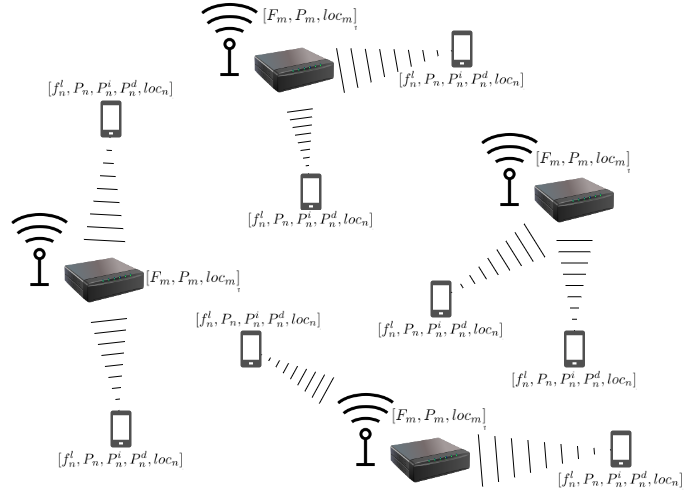
\includegraphics[width=\textwidth]{images/proposed_network.png}
  \caption{Proposed network model.} \label{proposed_network}
\end{figure}

The set of \acrshort{UE} is denoted as $\mathcal{N} = \{1, 2, ..., N\}$ while the set of \acrshort{MEC} servers can be denoted as $\mathcal{M} = \{1, 2, ..., M\}$. For simplicity \acrshort{MEC} servers are assumed to be connected to the power grid so their energy consumption is ignored.
\begin{itemize}
    \item Each \acrshort{UE}, $n \in \mathcal{N}$ can be described by its computing capacity, $f_n^l$ (\acrshort{CPU} cycles per second), transmit power, $P_n$, idle power consumption, $P^i_n$, download power consumption, $P_n^d$, and location, $loc_n = (x_n, y_n, z_n)$. The UE, $n$, can then be described by the vector, $u_n = [f_n^l, P_n, P_n^i, P_n^d, loc_n]$, and the system's \acrshort{UE}s can be defined as the vector $\mathcal{U} = [u_1, u_2, ..., u_n]$.

    \item Each \acrshort{MEC} server, $m \in \mathcal{M}$, can be described by its computing capacity, $F_m$ (\acrshort{CPU} cycles per second), its transmit power, $P_m$, and its location $loc_m = (x_n, y_n, z_n)$. The \acrshort{MEC} server, $m$, can then be described by the vector, $s_m = [F_m, P_m, loc_m]$ and the system's \acrshort{MEC} servers can be defined as the vector $\mathcal{S} = [s_1, s_2, ..., s_n]$.

    \item At each time step each \acrshort{UE} is assumed to have a computation task to be completed. This task can either be computed locally or offloaded to one of the available \acrshort{MEC} servers. The offloading decision of each computation task is denoted as $\alpha_n \in \{0, 1, ..., M\}$, where $\alpha_n = 0$ means local computation and $\alpha_n \in \mathcal{M}$ means offloading the task to \acrshort{MEC} server $m = \alpha_n$. The total offloading decision can be defined as the decision vector $\mathcal{A} = [\alpha_1, \alpha_2, ..., \alpha_N]$ with a decision for each task.

    \item Each computation task, $R_n$, can be defined by an input data amount, $B_n$ (bits), an output data amount, $B_d$ (bits), the total number of \acrshort{CPU} cycles required to compute it, $D_n$ and the importance weights of time and energy costs, $I_n^t$ and $I_n^e$. The importance weights of the task must satisfy $0 \leq I_n^t \leq 1$, $0 \leq I_n^e \leq 1$ and $I_n^t + I_n^e = 1$. The task, $R_n$, can then be described by the vector, $R_n = [B_n, B_d, D_n, I_n^t, I_n^e]$ and the system's tasks can be defined as the vector $\mathcal{R} = [R_1, R_2, ..., R_N]$.


\end{itemize}

If the network manager decides to compute the task, $R_n$, of \acrshort{UE} $n$ locally then a local computation model can be defined by a local execution delay $T_n^l$ and an energy consumption $E_n^l$:

\begin{equation}
    T_n^l = \frac{D_n}{f_n^l},
\end{equation}

\begin{equation}
    E_n^l = z_n D_n,
\end{equation}

where $z_n$ represents the energy consumption per \acrshort{CPU} cycle and is set to $z_n = 10^{-27}(f_n^l)^2$ according to practical observations made in \cite{energycons}.

Based on the computation delay and energy consumption of task, $R_n$, a local cost can be calculated according to:

\begin{equation}\label{localCost}
    C_n^l = I_n^t T_n^l + I_n^e E_n^l .
\end{equation}

If the network manager decides to offload the computation to the \acrshort{MEC} server $m = \alpha_n$, then the offload computation model can be defined by an upload delay, $T_{n,t}^m$, an upload energy consumption, $E_{n,t}^m$, an offload execution delay, $T_{n,p}^m$, an idle energy consumption, $E_{n,p}^m$, a download delay, $T_{n,d}^m$ and its corresponding download energy consumption, $E_{n,d}^m$.

Firstly, the \acrshort{UE} $n$ must upload the input data, $B_n$ from the task $R_n$ to the decided \acrshort{MEC} server $m$. This upload has an associated delay defined as:

\begin{equation} \label{transmission_delay}
    T_{n,t}^m = \frac{B_n}{r_u},
\end{equation}

where $r_u$ is the uplink rate of \acrshort{UE} $n$ computed according to Equation (\ref{uploaddelay}) from \cite{taskclass1} and the distance, $d_n^m$, between the \acrshort{MEC} server $m$ and the \acrshort{UE} $n$ can be calculated using the euclidean norm between their locations.

\begin{equation} \label{distance_nm}
    d_n^m = ||loc_m - loc_n||_2
\end{equation}

This upload has an associated energy consumption:

\begin{equation} \label{transmission_energy}
    E_{n,t}^m = P_n T_{n,t}^m = \frac{P_n B_n}{r_u} .
\end{equation}

After the data is uploaded the \acrshort{MEC} server then computes the task resulting in a offload execution delay:

\begin{equation} \label{processing_delay}
    T_{n,p}^m = \frac{D_n}{f_m} ,
\end{equation}

where $f_m$ is the amount of the \acrshort{MEC} server, $m$, computation capacity, $F_m$, allocated to the offloaded task. To simplify the system the computation capacity of a \acrshort{MEC} server is equally divided by all tasks offloaded to it:

\begin{equation}
    f_m = \frac{F_m}{N_m},
\end{equation}

where $N_m$ is the number of tasks offloaded to \acrshort{MEC} server, $m$.

While the \acrshort{UE} waits for the task to be computed it stays idle which has an associated energy consumption:

\begin{equation} \label{idle_energy}
    E_{n,p}^m = P_n^i T_{n,p}^m = \frac{P_n^i D_n}{f_m}.
\end{equation}

Finally the computation results are downloaded to the \acrshort{UE} $n$ with an associated delay:

\begin{equation} \label{download_delay}
    T_{n, d}^m = \frac{B_d}{r_d},
\end{equation}

where $B_d$ is the size of the computation output and $r_d$ is the download rate of \acrshort{UE} $n$ according to the Equation (\ref{downloaddelay}) from \cite{taskclass1}.

This download step has an associated energy consumption that can be calculated according to:

\begin{equation} \label{download_energy}
    E_{n, d}^m = P_n^d T_{n, d}^m .
\end{equation}

By taking into account the delays defined in Equations (\ref{transmission_delay}), (\ref{processing_delay}) and (\ref{download_delay}), we can compute the total offload delay, $T_n^m$ as the sum of all delays:

\begin{equation}
    T_n^m = T_{n,t}^m + T_{n,p}^m + T_{n, d}^m .
\end{equation}

The total energy consumption of offloading to the \acrshort{MEC} server $m$, can be calculated by adding all energy consumptions defined in Equations (\ref{transmission_energy}), (\ref{idle_energy}) and (\ref{download_energy}):

\begin{equation}
    E_n^m = E_{n,t}^m + E_{n,p}^m + E_{n, d}^m .
\end{equation}

Based on the computation delay and energy consumption of offloading task $R_n$ to \acrshort{MEC} server $m$, a cost can be calculated according to:

\begin{equation}
    C_n^m = I_n^t T_n^m + I_n^e E_n^m .
\end{equation}

The cost of the offloading decision $\alpha_n \in \{0, 1, ..., M\}$ can be computed according to:

\begin{equation}
    C_n =
    \begin{cases}
        C_n^l & \alpha_n = 0             \\
        C_n^m & \alpha_n \in \mathcal{M}
    \end{cases} .
\end{equation}

The system's costs can be defined as the vector:

\begin{equation}
    \mathcal{C} = [C_1, C_2, ..., C_N].
\end{equation}


The mean cost of the \acrshort{MEC} system at each iteration can then be defined as:

\begin{equation} \label{C_mean}
    C_{mean} = \frac{\sum\limits_{n=1}^N C_n}{N}.
\end{equation}

The worst case cost of the \acrshort{MEC} system at each iteration can then be defined as:

\begin{equation}
    C_{max} = \max \ \mathcal{C}.
\end{equation}

This corresponds to the \acrshort{UE} that has the highest cost at each iteration.

\subsection{Problem formulation}
\noindent The offloading decision needs to be formulated in a way that can both optimize overall system performance while considering the worst case serviced \acrshort{UE}.

Given this, the weighted cost at each iteration can be defined as:

\begin{equation} \label{cost_function}
    C = W_{mean}*C_{mean} + W_{max}*C_{max}.
\end{equation}

By picking the importance weights of the costs that satisfy:
\begin{align*}
    0 \leq W_{mean} \leq 1, \\
    0 \leq W_{max} \leq 1,  \\
    W_{mean} + W_{max} = 1.
\end{align*}

The priorities of the system can be adjusted to satisfy both overall system performance and consider the worst case cost of the system.

The optimization function can then be defined with the objective of finding the offloading decision vector $\mathcal{A} = [\alpha_1, \alpha_2, ..., \alpha_n]$ that minimizes the weighted average of the mean and max cost of the system at each iteration:

\begin{mini*}|s|
    {\mathcal{A}}{C}
    {}{}
    \addConstraint{C1: \alpha_n \in \{0, 1, ..., M\}, \forall n \in \mathcal{N}}
\end{mini*}


\subsection{Solution} \label{solution}
\noindent Given the complex nature of the proposed problem and the lack of perfect knowledge of network conditions this thesis proposes to use a model-free \acrshort{DRL} agent to manage the network. This means that the network manager does not have access to the transition probability, $P(s_{t+1}|s_t, a_t)$, nor the reward function $R(s, a)$ and must learn them by experimenting on the environment.

To do this the problem is formulated as an \acrshort{MDP}, $<S, A, P, R>$:
\begin{itemize}
    \item $S=\{s=(\mathcal{R})\}$ is the state space, which contains all requested tasks, $\mathcal{R}$;
    \item $A=\{a=(\mathcal{A})\}$ is the action space, which contains the offloading decision vector for all tasks, $\mathcal{A}$;
    \item $P:S \times A \times S \rightarrow [0, 1]$ is the transition probability distribution $P(s_{t+1}|s_t, a_t)$;
    \item $R = -C(s,a)$ is the reward function, which is defined as the inverse of the system cost, $C(s,a)$, given that the agent will be trying to maximize the reward.
\end{itemize}

At each time step, $t$, this network manager takes a state, $s_t$, makes a decision, $a_t$, that results in the state, $s_{t+1}$, and a reward $r_t$. The goal is then finding the policy, $\pi$, that maximizes the expected return, $V_\pi(s)$ as defined in Equation (\ref{Vfunction}).

To achieve this, several \acrshort{DRL} algorithms were explored: \acrshort{DQN}, \acrshort{DDQN}, \acrshort{Dueling DQN} and \acrshort{A2C}. Given the advantages presented in Section \ref{A3C}, the \acrshort{A2C} algorithm was chosen. The pseudocode of the \acrshort{A2C} algorithm is presented in Algorithm \ref{algorithm:A2C}, as defined in \cite{a3c}. To solve the exploration vs exploitation dilemma, the \acrshort{A2C} algorithm uses Boltzmann exploration as defined in Section \ref{boltz}.

\begin{algorithm}
\caption{Advantage actor-critic - pseudocode for each actor-learner thread.} \label{algorithm:A2C}
\emph{// Assume global shared parameter vectors $\theta$ and $\theta_v$ and global shared counter T = 0}

\emph{// Assume thread-specific parameter vectors $\theta'$ and $\theta'_v$}

\textbf{repeat}

\qquad Reset gradients: $d\theta \leftarrow 0$ and $d\theta_v \leftarrow 0$

\qquad Synchronize thread-specific parameters: $\theta' = \theta$ and $\theta'_v = \theta_v$

\qquad $t_{start} = t$

\qquad Get state $s_t$

\qquad \textbf{repeat}

\qquad \qquad Perform $a_t$ according to policy $\pi(a_t | s_t; \theta')$

\qquad \qquad Receive reward $r_t$ and new state $s_{t+1}$

\qquad \qquad $t \leftarrow t + 1$

\qquad \qquad $T \leftarrow T + 1$

\qquad \textbf{until} terminal $s_t$ \textbf{or} $t-t_{start} == t_{max}$

\[
R = \begin{cases}
  0  & \text{for terminal $s_t$}\\
  V(s_t, \theta'_v) & \text{for non-terminal $s_t$// Bootstrap from last state}
\end{cases}
\]

\qquad \textbf{for} $i \in {t-1, ..., t_{start}}$ \textbf{do}

\qquad \qquad $R \leftarrow r_i + \gamma R$

\qquad \qquad Accumulate gradients wrt $\theta': d\theta \leftarrow d\theta + \nabla_{\theta'} log_\pi(a_i | s_i; \theta')(R-V(s_i; \theta'_v))$

\qquad \qquad Accumulate gradients wrt $\theta'_v: d\theta_v \leftarrow d\theta_v + d(R - V(s_i; \theta'_v))^2 / d\theta'_v$

\qquad \textbf{end for}

\qquad Perform synchronous update of $\theta$ using $d\theta$ and of $\theta_v$ using $d\theta_v$.

\textbf{until} $T > T_{max}$


\end{algorithm}

As a function approximator for $V(s_t | \theta_v)$ and $\pi(a_t | s_t; \theta)$ a single neural network with two dense hidden layers was used. The hidden layers consist of 256 neurons each using the $tanh$ activation function. 

The input layer of this model consists of the flattened state vector, $S$. Since the state vector is a vector of length $N$, for the number of tasks and each task is described by a 5 variable vector, $R_n = [B_n, B_d, D_n, I_n^t, I_n^e]$, the total length of the input vector is $5 \times N$. 

The output of the model consists of two parts. First a single linear output representing the value function, $V(s_t | \theta_v)$. Secondly a softmax output for each action dimension with one entry per action, representing the probability of selecting the action, $\pi(a_t | s_t; \theta)$. 

Since the agent must decide for each task ($N$), between local computation or offloading to one of the MEC servers ($M$), there are $N$ softmax functions with $M+1$ entries each, representing the possible actions. A diagram of the model is shown in Figure \ref{fig:model}.

\begin{figure}[H]
  \centering
  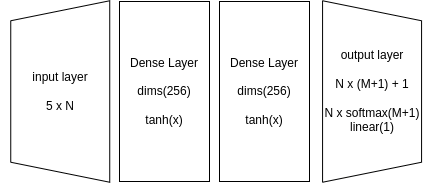
\includegraphics[scale=0.8]{images/model_arch.png}
  \caption{Model architecture.}
  \label{fig:model}
\end{figure}

\section{Methods and tools}

\noindent In order to implement a network manager capable of dealing with the proposed system two main challenges needed to be addressed: 1) the implementation of the \acrshort{DRL} algorithms; 2) the implementation of the proposed system simulator. The programming language that was used to implement all algorithms and the simulator is Python. The reason behind this decision is that given its popularity as the second most used programming language overall \cite{pythonpop} and the most used in the machine learning context \cite{pythonmachine}, most of all popular \acrshort{DRL} tools are written in Python.

As for the implementation of the \acrshort{DRL} algorithms two main tools were considered, Tensorflow 2.0 \cite{tensorflow} with the Keras API layer and Pytorch \cite{pytorch}. Due to the higher popularity of Tensorflow in the reinforcement learning context it was chosen as the neural network library used to write all DRL algorithms. To help with the distributed nature of some of the \acrshort{RL} algorithms the open-source library RLlib \cite{rllib} was used.

The second major challenge is the implementation of the simulator. OpenAI Gym was introduced in \cite{opengym} in order to standardize reinforcement learning environments and benchmarks. Due to its easy integration with Keras demonstrated in \cite{kerasrl} and \cite{kerasrl2} it was chosen as the tool for implementing the simulation environment of the proposed system.